
The Hazard function of $X$,
\begin{align}
\lambda(X) = \frac{f(x)}{S(x)} \label{var/1/eq:1}
\end{align}
where $S(x)$ is the survival function given by,
\begin{align}
S(x) = P(X \geq x) = 1-F(x) = \int_{x}^{\infty}f(t)dt
\end{align}
\begin{lemma}
\begin{align}
S(x)=
\begin{cases}
e^{-(x-\mu)^\alpha} &x>\mu\\
1 &x\leq\mu
\end{cases}
\end{align}
\end{lemma}
\begin{proof}

\begin{align}
\int f(t)dt=\int \alpha(t-\mu)^{\alpha-1}e^{-(t-\mu)^\alpha}dt\\
=-e^{-(t-\mu)^\alpha} + C
\end{align}
If $x>\mu$, 
\begin{align}
S(x) = \int_{x}^{\infty} \alpha(t-\mu)^{\alpha-1}e^{-(t-\mu)^\alpha}dt\\
=-e^{-(t-\mu)^\alpha}]_{x}^{\infty}\\
=e^{-(x-\mu)^{\alpha}} \label{var/1/eq:2}
\end{align}
If $x\leq\mu$,
\begin{align}
S(x) = \int_{x}^{\mu}f(t)dt + \int_{\mu}^{\infty}f(t)dt\\
     = 0 + e^{-(\mu-\mu)^{\alpha}}\\
     =1 \label{var/1/eq:3}
\end{align}
From \eqref{var/1/eq:2} and \eqref{var/1/eq:3}, we get $S(x)$ as,
\begin{align}
S(x)=
\begin{cases}
e^{-(x-\mu)^\alpha} &x>\mu\\
1 &x\leq\mu \label{var/1/eq:4}
\end{cases}
\end{align}
\end{proof}
From \eqref{var/1/eq:1} and \eqref{var/1/eq:4}, we get
\begin{align}
\lambda(x) = 
\begin{cases}
\alpha(x-\mu)^{\alpha-1} &x>\mu\\
0 &x\leq\mu \label{var/1/eq:5}
\end{cases}
\end{align}
So,\\ if $\alpha>1$, $\lambda(x)$ is an increasing function
\begin{figure}[htp]
    \centering
    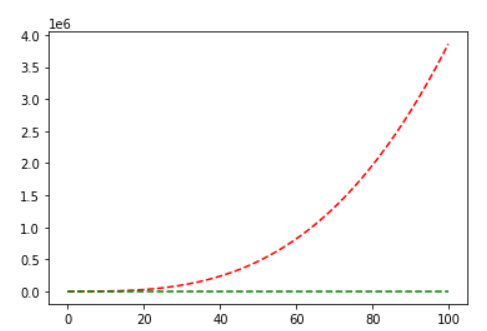
\includegraphics[width=\columnwidth]{variable/solutions/1/alphagrt1.png}
    \caption{$\alpha=2$ for red. $\alpha=1$ for green, $\mu=1$ for both}
    \label{var/1/fig:grt1}
\end{figure}
and\\ if $0<\alpha<1$, $\lambda(x)$ is a decreasing function
\begin{figure}[htp]
    \centering
    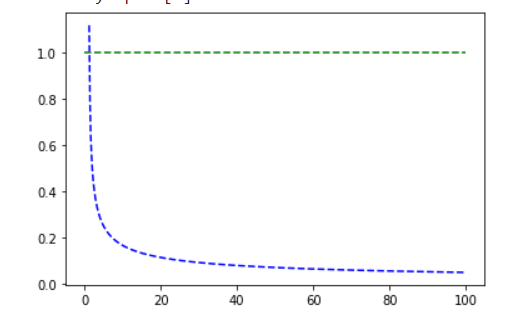
\includegraphics[width=\columnwidth]{variable/solutions/1/alphales1.png}
    \caption{$\alpha=0.5$ for blue. $\alpha=1$ for green, $\mu=1$ for both}
    \label{var/1/fig:les1}
\end{figure}
and\\ for $\alpha=1$, $\lambda(x)=1$, a constant function.\\
So, for some values of $\alpha$, it is increasing, for some it is decreasing function\\
\textbf{Therefore, answer is (C) and (D)}
